% generated by Docutils <http://docutils.sourceforge.net/>
\documentclass[t,english]{beamer}
\usepackage{hyperref}

\definecolor{rrblitbackground}{rgb}{0.55, 0.3, 0.1}

\newenvironment{rtbliteral}{

\begin{ttfamily}

\color{rrblitbackground}

}{

\end{ttfamily}

}

\usetheme{Warsaw}

\setbeameroption{hide notes}

\usepackage{fixltx2e} % LaTeX patches, \textsubscript
\usepackage{cmap} % fix search and cut-and-paste in PDF
\usepackage{babel}
\usepackage[T1]{fontenc}
\usepackage[latin1]{inputenc}
\usepackage{ifthen}
\usepackage{graphicx}

%%% User specified packages and stylesheets

%%% Fallback definitions for Docutils-specific commands

% hyperlinks:
\ifthenelse{\isundefined{\hypersetup}}{
  \usepackage[colorlinks=true,linkcolor=blue,urlcolor=blue]{hyperref}
}{}
\hypersetup{
  pdftitle={Introduction to PSoCs},
}

%%% Body
\begin{document}

% Document title
\title{Introduction to PSoCs%
  \phantomsection%
  \label{introduction-to-psocs}}
\author{}
\date{}
\maketitle

\begin{frame}
\frametitle{What is a PSoC?}

\begin{columns}[T]
\column{0.47\textwidth}
\begin{itemize}[<+-| alert@+>]

\item Micro-controller

\item programmable in C or assembly

\item 24 MHz

\item 32 kB Flash ROM

\item 2 kB SRAM

\item connection pins

\item Cost: < \$10 (chip)

\item \$130 for the eval board w/chip
\end{itemize}

\column{0.47\textwidth}

\noindent\makebox[\textwidth][c]{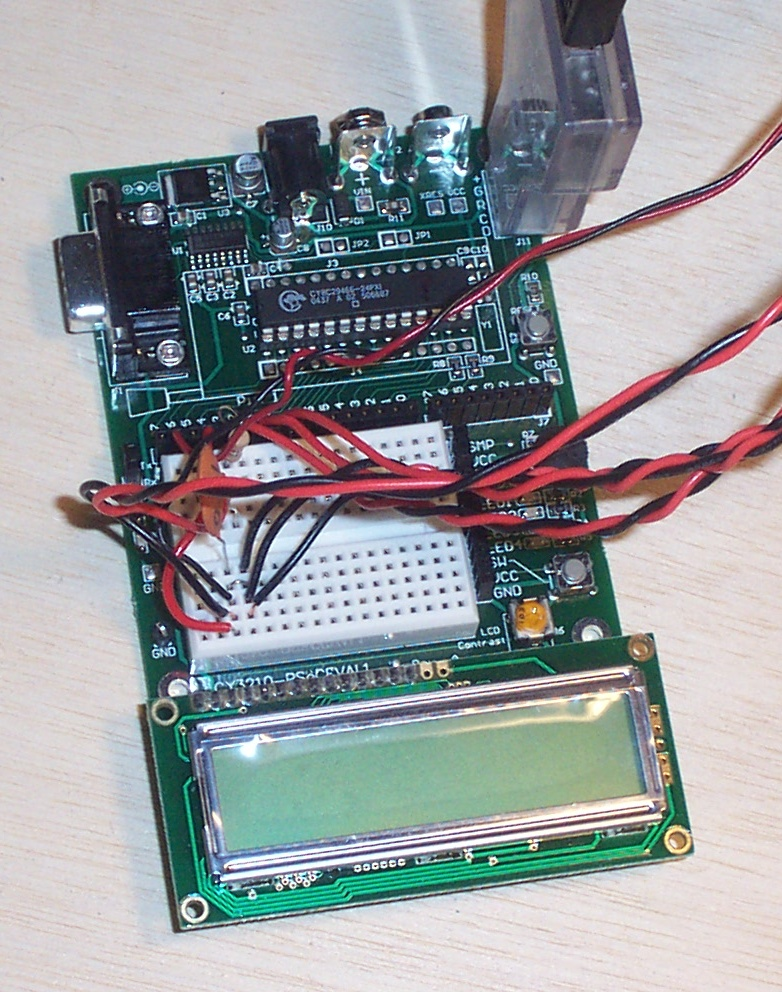
\includegraphics[width=1.85in]{PSoC_06_cropped}}

\end{columns}
\end{frame}

\begin{frame}
\frametitle{Why micro-controllers?}

\begin{itemize}[<+-| alert@+>]

\item cheap

\item small

\item put them in anything

\item \$12 billion/year industry
\end{itemize}
\end{frame}

\end{document}
